\RequirePackage{scrlfile}
\ReplacePackage{scrpage2}{scrlayer-scrpage}
\documentclass[paper=a4,toc=bibliography,chapterprefix,parskip=true]{scrreprt}

% -------------------------------------------------------------------
%%% Laden elementarer Pakete
%
% Deutsche Schriftpakete
\usepackage[utf8]{inputenc}              % alternativ: 'ansinew' oder 'latin9' statt utf8
\usepackage[TS1,T1]{fontenc}
\usepackage{lmodern,textcomp}
\usepackage[english,ngerman]{babel}
%
% Mathematische Paktete
\usepackage{amsmath,amssymb,bm,bbm}         % Formelsetzung und mathematischen Symbole
\usepackage[amsmath,thmmarks]{ntheorem}     % Theorem-Umgebungen, alternativ: 'amsthm'
%
% Grafik-Pakete einbinden
\usepackage{graphicx,psfrag}                % Basis-Pakete zum Laden von Bildern (jpg?)
\usepackage{float}
\usepackage{color}                          % erweitertes Farb-Paket, alternativ: 'xcolor'
\usepackage{tikz}
\usepackage{pgfplots}
%\usepackage{pstricks,pst-plot}              % weiteres Paket zur Erstellung von LaTeX-Grafiken
%
% erweiterte Tabellen
\usepackage{array}                          % Basis-Paket
\usepackage{booktabs}                       % 'schöne' Tabellen
\usepackage{tabularx}                       % Tabellen mit dynamischer Spaltenbreite
\usepackage{longtable}                      % Tabellen mit möglichem Seitenumbruch
\usepackage{multirow}                       % mehrzeilige Zellen
%
% weitere
\usepackage{verbatim, listings}             % Darstellung von Quellcode
\lstset{language=TeX,basicstyle=\footnotesize,frame=single,breaklines=true}
\usepackage[format=plain,indention=.5cm]{caption} % für selbsdefinierte captions
\usepackage{stmaryrd}                       % Blitzsymbol bei Widerspruch
%\usepackage[square]{natbib}                 % naturwissenschaftliche Zitierweise
%
% Paket für interne Links
\usepackage[%
	breaklinks=true    % Links »überstehen« Zeilenumbruch
	,colorlinks        % Links erhalten Farben statt Kästen
	,linkcolor=black   % beeinflusst Inhaltsverzeichnis und Seitenzahlen
	,urlcolor=black    % Farbe für URLs
	,citecolor=black
	,bookmarks         % Erzeugung von Bookmarks für PDF-Viewer
	,bookmarksnumbered % Nummerierung der Bookmarks
]{hyperref}
\usepackage{breakurl}
%
% -------------------------------------------------------------------


% -------------------------------------------------------------------
%%% Seitenstil
%
\usepackage{scrpage2}                       % Kopf- und Fußzeilenformatierung
\usepackage[onehalfspacing]{setspace}       % Zeilenabstand = 1,5
\recalctypearea
\pagestyle{scrheadings}
\automark[section]{chapter}
\addtokomafont{sectioning}{\rmfamily}
%
% -------------------------------------------------------------------


% -------------------------------------------------------------------
%%% Einstellungen und Formatierung der Theorem-Umgebung
%
% Stil der Definition - Umgebung
\theoremstyle{break}
\theoremheaderfont{\sffamily\bfseries}
\theorembodyfont{\upshape}
\theoremsymbol{}
\newtheorem{definition}{Definition}[chapter]
\newtheorem{satz}[definition]{Satz}
\newtheorem{resultat}[definition]{Resultat}
\newtheorem{lemma}[definition]{Lemma}
\newtheorem{folgerung}[definition]{Folgerung}
\newtheorem{korollar}[definition]{Korollar}
%
\theorembodyfont{\rmfamily}
\newtheorem{bemerkung}[definition]{Bemerkung}
\newtheorem{beispiel}[definition]{Beispiel}
%
% Stil der Beweis - Umgebung
\theoremstyle{nonumberplain}
\theoremsymbol{\ensuremath{\Box}}
\newtheorem{beweis}{Beweis}
%
% ------------------------------------------------------------------- 

\begin{document}

% -------------------------------------------------------------------
% Titelseite, Inhaltsverzeichnis, Abbildungsverzeichnis, usw.

\begin{titlepage}
	\begin{center}
		{\LARGE \textsc{Technische Universität Dortmund}} \\[4ex]
		{\Large Fakultät Informatik\\
		Design Automation for Embedded Systems Group \\}
	\end{center}
  \vspace*{8ex}
  \begin{center}
    {\Huge \textbf{~\\
    TODO Titel} \\}
  \end{center}
  \vspace*{8ex}
  \begin{center}
  	{\huge \textsc{Fachprojekt} \\[6ex] }
    {\Large Jack Diep, Florian Köhler, Yannick Naumann \\}
    \end{center}
    \vspace*{8ex}
	\begin{flushleft}
        {\large
		Betreuung: \\
		M.Sc. Mikail Yayla \\
		\vspace*{4ex}
		\today \\}
	\end{flushleft}	
\end{titlepage}
 % <- Hier sollten Name/Titel/usw. eingetragen werden!
\pagenumbering{roman}
\tableofcontents
\listoffigures
\addcontentsline{toc}{chapter}{Abbildungsverzeichnis}
%\listofalgorithms
% ...
\clearpage
\pagenumbering{arabic}
% -------------------------------------------------------------------

% -------------------------------------------------------------------
% Hauptteil
\chapter{Einleitung}

Neuronale Netzwerke bilden eine Unterkategorie des Machine-Learning und erlauben
Auswertungen von Eingaben auf Basis von zuvor angelernten, empirischen
Ergebnissen.
Ein neuronales Netzwerk bildet ein System aus Neuronen ab, welche Schichtweise
verbunden sind einen unidirektionalen Datenfluss erzeugen.
Dieses System besteht üblicherweise aus einer Eingabeschicht, einer
Ausgabeschicht und dazwischen beliebig viele \emph{versteckte} Schichten,
welche die eigentliche Arbeit des Netzwerks verrichten.
Die Anzahl der Neuronen in den Eingabe- und Ausgabeschichten ist intuitiv
wählbar. Die Größe der Eingabeschicht wird häufig durch die Anzahl der
möglichen Eingaben bestimmt, die Größe der Ausgabeschicht durch die Anzahl
der möglichen Ergebnisse.
Die Größe und Anzahl der dazwischen liegenden Schichten hingegen muss je
nach Anforderung und Gegebenheiten individuell ermittelt werden.
Je größer das Netzwerk desto höher sind die Anforderungen an die benötigte
Hardware um dieses zu betreiben. Bei schwächerer Hardware oder
Einschränkungen bezüglich der Energieversorgung können kleinere Netzwerke
eingesetzt werden, wenn auch häufig mit geringerer Genauigkeit verglichen
mit einem größeren Netzwerk.


\section{Motivation}

Die Größe eines Netzwerks kann beim Entwurf dessen direkt beeinflusst werden.
In Anwendungsgebieten, bei denen der Fokus auf geringen Hardwareanforderungen
liegt, stoßen schnell das Problem der schwindenden Genauigkeit.
Auf IoT-Geräten oder mobilen Platformen finden klassische neuronale Netzwerke
daher nur eingeschränkt Nutzen.
2016 veröffentlichten M. Courbariaux und Y. Bengio \cite{Courbariaux} eine 
wissenschaftliche Arbeit und stellen dort das
\emph{binarisierte neuronale Netzwerk} (kurz BNN) vor.
Dieses könne im Vergleich zu einem klassischen neuronalen Netzwerk eine
theoretische Geschwindigkeitssteigerung auf das 32-fache erreichen.
Die Genauigkeit des BNN liege jedoch nur knapp unter derer klassischer Netzwerke.
Das BNN ermöglicht dank dieser Eigenschaften den Einsatz von neuronalen Netzen
auf vergleichsweise schwacher Hardware und verspricht zugleich
nur geringe Genauigkeitseinbüße.

In dieser Ausarbeitung wird die allgemeine Funktionsweise von neuronalen
Netzwerken erläutert und anschließend der Entwurf eines binarisiertes
Netzwerk mit Fokus auf Handschriftenerkennung auf Basis des MNIST Datensatzes
dokumentiert.
Dabei werden grundlegende Überlegungen, das Vorgehen, Herausforderungen
sowie dazu erarbeitete Lösungen vorgestellt.
\chapter{Neuronale Netzwerke}

Unter einem neuronalen Netzwerk versteht man ein System
aus Neuronen. Diese sind schichtweise organisiert wobei
jedes Neuron einer Schicht jeweils zu allen Neuronen der
direkt anliegenden Schichten verbunden ist.
Abbildung \ref{fig:Neuronales Netzwerk} zeigt beispielhaft ein
neuronales Netzwerk aus 19 Neuronen mit insgesamt 5 Schichten.
\bigskip

\begin{figure}[h]
    \begin{center}
        \begin{tikzpicture}[y=-1.5cm,x=3cm]
            \tikzset{
                netnode/.style={circle,draw=black,minimum size=1cm},
                hidden/.style={dotted,thick}
            }
            \node[netnode] (i1) at (0,0) {$i_1$};
            \node[netnode] (i2) at (0,1) {$i_2$};
            \node[netnode] (i3) at (0,2) {$i_3$};

            \node[netnode,hidden] (l11) at (1,-1) {};
            \node[netnode,hidden] (l12) at (1,0) {};
            \node[netnode,hidden] (l13) at (1,1) {};
            \node[netnode,hidden] (l14) at (1,2) {};
            \node[netnode,hidden] (l15) at (1,3) {};

            \node[netnode,hidden] (l21) at (2,-0.5) {};
            \node[netnode,hidden] (l22) at (2,0.5) {};
            \node[netnode,hidden] (l23) at (2,1.5) {};
            \node[netnode,hidden] (l24) at (2,2.5) {};

            \node[netnode,hidden] (l31) at (3,-1) {};
            \node[netnode,hidden] (l32) at (3,0) {};
            \node[netnode,hidden] (l33) at (3,1) {};
            \node[netnode,hidden] (l34) at (3,2) {};
            \node[netnode,hidden] (l35) at (3,3) {};

            \node[netnode] (o1) at (4,0.5) {$o_1$};
            \node[netnode] (o2) at (4,1.5) {$o_2$};

            \foreach \i in {1,2,3}{
                    \foreach \j in {1,...,5}{
                            \draw[->,black!25] (i\i) -- (l1\j);
                        }
                }
            \foreach \i in {1,...,5}{
                    \foreach \j in {1,...,4}{
                            \draw[->,black!25] (l1\i) -- (l2\j);
                        }
                }
            \foreach \i in {1,...,4}{
                    \foreach \j in {1,...,5}{
                            \draw[->,black!25] (l2\i) -- (l3\j);
                        }
                }
            \foreach \i in {1,...,5}{
                    \foreach \j in {1,2}{
                            \draw[->,black!25] (l3\i) -- (o\j);
                        }
                }
        \end{tikzpicture}
    \end{center}
    \caption{Struktur eines neuronalen Netzwerks}
    \label{fig:Neuronales Netzwerk}
\end{figure}

\section{Neuronen}

Unter einem Neuron versteht sich bei neuronalen Netzen lediglich ein Knoten,
in dem üblicherweise ein 32-bit großer Wert hinterlegt ist. Häufig kommen hier
Gleitkommazahlen zwischen -1.0 und 1.0 zum Einsatz, da sich dieser Wertebereich
besonders gut zum Rechnen eignet und Eigenschaften bezüglich der
Multiplikation besitzt, die eine Wertexplosion verhindern.
Die Werte aller Neuronen, mit Ausnahme derer in der Eingabeschicht, setzen sich
jeweils aus den Werten aller Neuronen der direkt davor liegenden Schicht zusammen.
Das genaue Vorgehen bei der Wertermittlung hängt jeweils vom Netzwerk
und den dort verwendeten Aktivierungsfunktionen ab.

\section{Schichten und Kanten}

In einem neuronalen Netzwerk ist jedes Neuron einer Schicht mit allen Neuronen
der jeweiligen davor liegenden und danach liegenden Schicht über Kanten verbunden.
Neuronale Netzwerke sind unidirektionale Graphen, demnach fließen Informationen
über Schichten (und folglich Kanten) nur in eine Richtung.

Allen Kanten wird initial eine Gewichtung zugewiesen, welche erneut
netzwerkabgängig generiert werden oder durch zuvor angelernte Daten bestimmt
werden. Beim Trainieren des Netzwerks werden diese bei jeder Lerniteration
(auch \emph{Epoch} genannt) justiert, während sie beim Betrieb für gewöhnlich
keine Änderungen mehr erfahren.
Die Genauigkeit eines Netzwerks wird überwiegend durch diese Gewichte bestimmt,
daher ist das Ziel beim Trainieren eines Netzes die Optimierung jener.

Kantengewichte wirken sich maßgeblich auf die Wertberechnung von Neuronen aus.
Diese wird in zwei Schritten ausgeführt. Im ersten Schritt wird aus den
Kantengewichten aller eingehenden Kanten und den Werten der darüber
verbundenen Neuronen die Produktsumme gebildet.
Für den zweiten Schritt sind jeweils Aktivierungsfunktionen notwendig, welche
im nachfolgenden Kapitel erläutert werden.

\section{Aktivierungsfunktionen}

Im zweiten Schritt wird der zuvor errechnete Wert durch eine weitere Funktion
modifiziert. Sogenannte \emph{Aktivierungsfunktionen} können beliebig gewählt
werden, müssen jedoch offensichtlich alle möglichen Eingaben auf einen Wert
abbilden können. Die verwendete Aktivierungsfunktion kann je nach
Schicht variieren. Einmal gewählt, ist diese jedoch für die jeweilige Schicht
im Netzwerk für die Laufzeit fest.

Die beiden erläuterten Berechnungsschritte werden schichtweise in Richtung des
Datenflusses des Netzwerks für alle Neuronen durchgeführt. Im folgenden
Beispiel wird bildhaft dargestellt, wie solch eine Neuronenwertberechnung für
ein Netzwerk aussieht, welche in der betrachteten Schicht die
$tanH$-Aktivierungsfunktion verwendet.

\begin{figure}
    \centering
    \begin{tikzpicture}[y=-1.5cm,x=1.5cm]
        \tikzset{
            netnode/.style={circle,draw=black,minimum size=1cm},
            hidden/.style={dotted,thick}
        }
        \node[netnode] (i1) at (0,0) {0.7};
        \node[netnode] (i2) at (0,1) {0.5};
        \node[netnode] (i3) at (0,2) {-0.2};
        \node[netnode] (i4) at (0,3) {-0.9};

        \draw[draw=black,dotted] (-0.5,-1) rectangle ++(1,5) ++(-0.5,0) node[below] {Schicht $n$};
        \draw[draw=black,dotted] (2,-1) rectangle ++(5,5) ++(-2.5,0) node[below] {Schicht $n+1$};

        \node[netnode,minimum size=2cm,dotted,thick] (o1) at (3,1.5) [label=below:Schritt 1] {$=0.67$};
        \node (o1l) [above of=o1,align=right,above] {$0.7\times 0.6$\\$+\ 0.5\times 0.7$\\$+\ 0.2\times 0.4$\\$-\ 0.9\times 0.2$};

        \node[netnode,minimum size=2cm] (o2) at (6,1.5) [label=below:Schritt 2] {$\approx 0.585$};

        \draw[->] (i1) -- node[auto] {0.6} (o1);
        \draw[->] (i2) -- node[auto] {0.7} (o1);
        \draw[->] (i3) -- node[auto] {-0.4} (o1);
        \draw[->] (i4) -- node[auto] {0.2} (o1);
        \draw[->,dotted,thick] (o1) -- node[above] {$tanH(x)$} (o2);
    \end{tikzpicture}
    \caption{Berechnung eines Neuronenwertes\\mit der $tanH$ Aktivierungsfunktion}
\end{figure}

Die Wahl der Aktivierungsfunktion beeinflusst die möglichen
Werte, die Neuronen innerhalb einer Schicht annehmen können. Um eine
Wertexplosion zu vermeiden (z.B. bei Verwendung von $ReLU(x): \max(0,x)$ als
Aktivierungsfunktion), können zusätzliche Normalisierungsschichten verwendet
werden, welche die Neuronenwerte einer Schicht auf einen erwünschten Zielbereich
einschränken. Es existieren jedoch auch Aktivierungsfunktionen, die diese
\emph{Squashing-}Eigenschaft direkt besitzen. Darunter zählt auch die im
vorherigen Beispiel verwendetete Funktion $tanH$, bei der alle Eingaben auf den
Zielbereich [-1,1] abgebildet werden.

Im Folgenden sind sind einige, für neuronale Netzwerke übliche
Aktivierungsfunktionen abgebildet.

\begin{figure}[H]
    \begin{minipage}{0.45\textwidth}
        \begin{center}
            \begin{tikzpicture}
                \begin{axis}[width=7cm,xmin=-5,xmax=5,ymin=-2,ymax=2,thick,grid=both]
                    \addplot[] {max(x,0))};
                \end{axis}
            \end{tikzpicture}
        \end{center}
        \caption{ReLU}
    \end{minipage}\hfill
    \begin{minipage}{0.45\textwidth}
        \begin{center}
            \begin{tikzpicture}
                \begin{axis}[width=7cm,xmin=-5,xmax=5,ymin=-2,ymax=2,thick,grid=both]
                    \addplot[] {1/(1+exp(-x))};
                \end{axis}
            \end{tikzpicture}
        \end{center}
        \caption{Sigmoid}
    \end{minipage}
\end{figure}
%
\begin{figure}[H]
    \begin{minipage}{0.45\textwidth}
        \begin{center}
            \begin{tikzpicture}
                \begin{axis}[width=7cm,xmin=-5,xmax=5,ymin=-2,ymax=8,thick,grid=both]
                    \addplot[] {x};
                \end{axis}
            \end{tikzpicture}
        \end{center}
        \caption{Softmax}
    \end{minipage}\hfill
    \begin{minipage}{0.45\textwidth}
        \begin{center}
            \begin{tikzpicture}
                \begin{axis}[width=7cm,xmin=-5,xmax=5,ymin=-2,ymax=2,thick,grid=both]
                    \addplot[] {(exp(x)-exp(-x)) / (exp(x)+exp(-x))};
                \end{axis}
            \end{tikzpicture}
        \end{center}
        \caption{tanH}
    \end{minipage}
\end{figure}

\section{Training}

Die Stärken und Schwächen eines neuronalen Netzwerks liegen neben der
Struktur der Neuronen, der Schichten und den gewählten Aktivierungsfunktionen
vor allem in den verwendeten Kantengewichten. Diese zu optimieren kann ein
langwieriger und rechenintensiver Prozess sein. Kleine Änderungen im Aufbau
des Netzwerks können große Teile von zuvor erlernten Gewichten unbrauchbar
machen, daher werden Netzwerke häufig an sich selbst trainiert.
Das bedeutet, dass beim Trainieren eines neuen Netzwerks die initialen
Kantengewichte keine emprischen Daten aus anderen (ähnlichen) Netzwerk verwenden,
sondern diese zu Beginn pseudozufällig gewählt werden.

\subsection{Ablauf}

\subsection{Backpropagation (?)}


\chapter{Das Netzwerk}
\section{Aktivierungsfunktion}
\section{Binärer Linear-Layer}
\section{Verluste durch binäre Linear-Layer}
Durch die binarisierung der \textit{Linear-Layer} ist zu vermuten, dass diese, im Vergleich zu normalen \textit{Linear-Layer}, etwas schlechter performen. Dies ist der Fall, da die Anzahl der möglichen Kantengewichte stark, auf Null und Eins, eingeschränkt ist. 
%TODO konkrete Messung

Trainiert wurde hier das gleiche Netzwerk, ein mal mit binären \textit{Linear-Layern}, das andere mal mit normalen \textit{Linear-Layer}. Jedes Netzwerk wurde für 50 Epochen trainiert, bevor die Genauigkeit ausgewertet wurde. Um sicher zu gehen, ob die Genauigkeit gegen diesen Wert konvergiert, wurde jede Messung fünf mal wiederholt.
\chapter{Training des BNNs}
Wie bereits in Kapitel \ref{sec:training} beschrieben, werden Netzwerke über eine rechenintensive Annäherung der Kantengewichte an das optimale Ergebnis trainiert. Diese Konvergenz in Richtung eines besseren Ergebnisses kann hierbei, selbst bei schlechtem Training, meist erreicht werden, da selbst marginale Verbesserungen eine Auswirkung haben. Da \textit{BNNs} jedoch die stärkste Form von quantisierten Netzwerken sind, können hier keine stetigen Änderungen an den Kantengewichten vorgenommen werden.
\section{Lernrate}
Die Lernrate ist ein zentrales Parameter beim Training von Neuronalen Netzwerken. Sie gibt die Rate an, mit der Kantengewichte in einem Durchlauf angepasst werden. Je höher die Lernrate also ist, desto schneller passt sich das Model an gerade trainierte Daten an. Bei der Wahl der Rate sind die Probleme des \textit{overfitting} und \textit{underfitting} zu beachten.\\ 
Als \textit{undefitting} bezeichnet man eine zu geringe Anpassungsfähigkeit des Netzwerkes, ausgelöst über zu kleine Netze oder zu niedrige Lernrate. Ist die Lernrate zu klein, kann der Error nicht reduziert werden, die Genauigkeit nimmt nur, wenn überhaupt, sehr langsam zu. Das Netz kann aus Daten keine Lernerfolge ziehen.\\
\textit{Overfitting} ist eine zu schnelle Anpassung des Models. Ist zum Beispiel die Lernrate zu hoch, kann die optimale Genauigkeit des Netzwerkes nicht erreicht werden, da die Anpassungen pro Trainingsdatum zu groß sind. Hier wird das Optimum immer, durch eine Überkorrektur, übersprungen und kann nie erreicht werden\cite{smith2018}. Diese Probleme sind hier analog zu \textit{vanishing-} beziehungsweise \textit{exploding gradient}.

\begin{figure}[H]
	\centering
	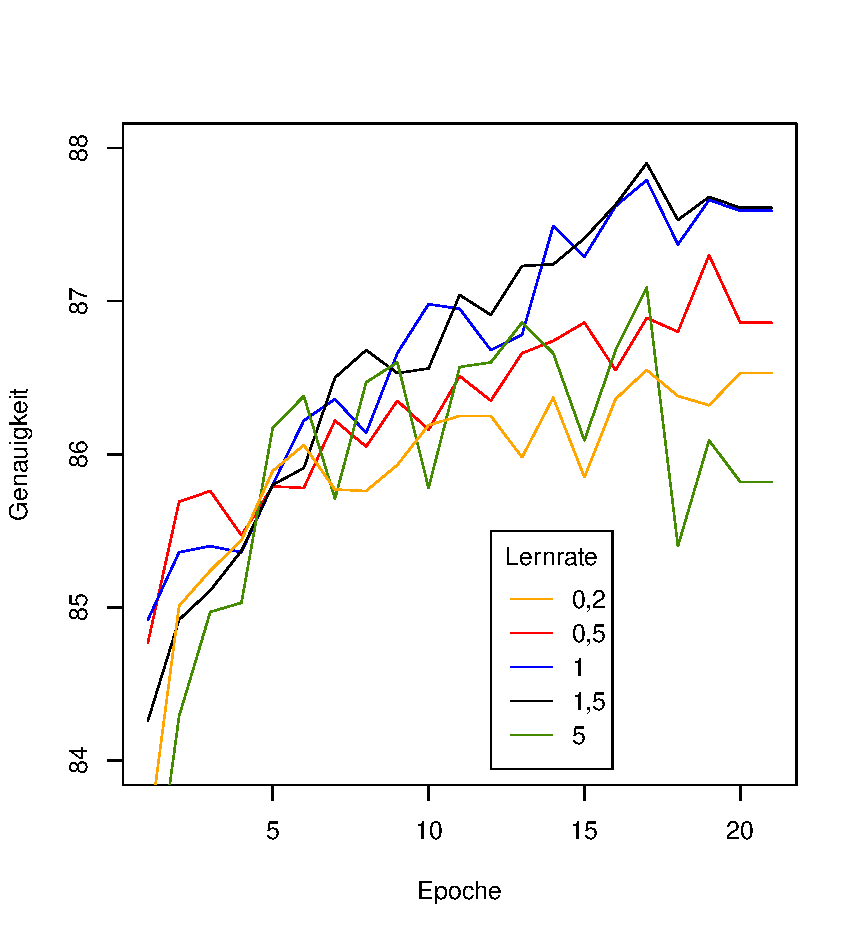
\includegraphics[scale=0.9]{./bilder/learningrate}
	\caption{Training mit verschiedenen Lernraten}
	\label{fig:learningrate}
\end{figure}

Zur Ermittlung der optimalen Lernrate haben wir unser Netzwerk für 20 Epochen mit verschiedenen Lernraten trainieren lassen. In Abbildung \ref{fig:learningrate} sind die Ergebnisse mit einer Messung der Genauigkeit nach jeder Epoche dargestellt. Bei einer Lernrate von 5 ist deutlich eine Überkorrektur ab Generation 17 zu erkennen. Hier werden zu starke Anpassungen vorgenommen, weshalb sich die Genauigkeit vom Optimum entfernt. Lernraten unter Eins hingegen nähern sich dem Optimum erst gar nicht genug an. Hier ist ein potentieller \textit{vanishing gradient} zu erkennen, da der Error nicht signifikant sinkt.  Die Lernraten 1 und $1,5$ liefern hier die besten Ergebnisse. Da das Training mit einer Rate von $1,5$ weniger große Ausschläge zeigt, wurde sich für diese Lernrate entschieden.
\section{Batchgröße}
Die Batchgröße hat Einfluss auf mehrere Punkte des Netzwerkes. Zum Einen entscheidet sie, wie viele Daten durch das Netzwerk laufen, bevor der Error gemessen wird und die Gewichte aktualisiert werden. Zum Anderen wirkt sich dies auf die BatchNorm Schicht aus. Je größer hier die Batchgröße ist, desto stärker ist die Normalisierung durch die BatchNorm.

\begin{figure}[H]
	\centering
	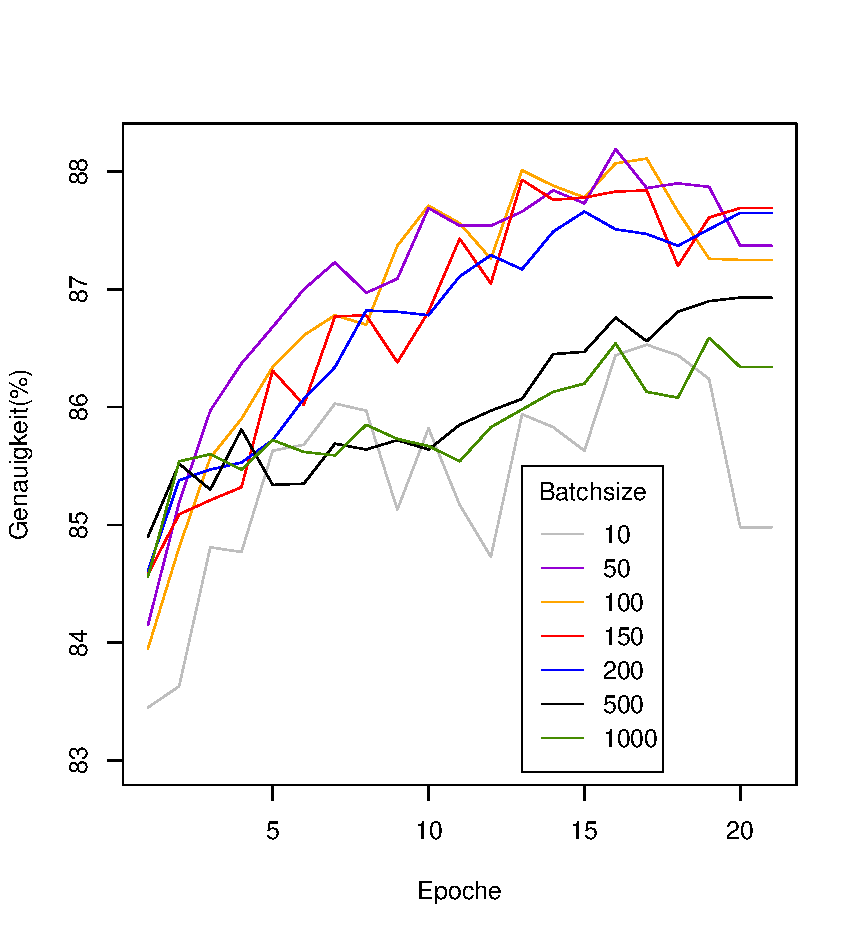
\includegraphics[scale=0.9]{./bilder/batchsize_measurement}
	\caption{Training mit verschiedenen Batchgrößen}
	\label{fig:batchsize}
\end{figure}
In Abbildung \ref{fig:batchsize} zu sehen ist das immer gleiche Netzwerk, lediglich mit angepasster Batchgröße. Dieses Netzwerk wurde für 20 Epochen beobachtet.\\
Auffällig ist die stark ausschlagende Kurve bei einer Batchgröße von 10. Hier ist der Wert zu gering, weshalb der Error oft berechnet wird. Da außerdem wenig über die BatchNorm normalisiert wird, kommt es zu hohen Error-Werten und starken und häufigen Anpassungen des Netzwerkes.\\
Bei einer Batchgröße $\geq 500$ sind weniger starke Ausschläge zu beobachten. Allerdings ist hier zu beobachten, dass das Netzwerk nicht mehr so Effizient trainiert wie bei kleineren Batchgrößen. Hier könnte die Normalisierung und damit die Generalisierung bereits zu stark sein. Außerdem wird hier der Error wesentlich seltener berechnet und das Netzwerk ist somit wesentlich unagiler. Es kommt zum \textit{underfitting}.\\
Bei Batchgrößen 50-200 ist keine besondere Abweichung zu erkennen, wobei 50 und 100 am besten performen.
\begin{figure}[H]
	\centering
	\begin{tabular}{|c|c|c|c|c|c|c|c|}\hline
		Batchgröße&10&50&100&150&200&500&1000\\\hline
		Zeit (s)&30,68&11,33&8,76&7,95&7,63&6,66&6,39\\\hline
	\end{tabular}
	\caption{Zeit pro Epoche für verschiedene Batchgrößen }
	\label{fig:batchsize_time}
\end{figure}
Ein weiterer, praxisrelevanter, Faktor ist, dass das Training mit größeren Batchgrößen schneller geht. Da mehr Daten parallel bearbeitet werden, ist die gleiche Anzahl an Daten schneller abgearbeitet. In Abbildung \ref{fig:batchsize_time} sind die Zeiten für eine einzige Epoche, abhängig von der jeweiligen Batchgröße, gelistet. Es ist zu erkennen, dass besonders kleine Batchgrößen bei einer Erhöhung Zeiteinsparungspotential haben. Da die Werte 50-200 bei der Genauigkeit am besten abgeschnitten haben und $t(100)-t(50) <t(200)-t(100)$, ist hier die Laufzeitverbesserung von 50 auf 100 eine Sinnvolle Einsparung. Bei Batchgrößen $\geq 150$ lohnt sich die marginale Zeiteinsparung im Vergleich zur schlechteren Genauigkeit nicht mehr.\\
Deshalb haben wir uns für ein Batchgröße von 100 zur optimalen Werteberechnung entschieden.


\chapter{Binarisierung}



\chapter{Export}
Nachdem das Netzwerk nun trainiert wurde, müssen die Ergebnisse, die Kantengewichte und Schwellwerte der Neuronen, nun exportiert werden. Im Folgenden sollen diese dann in den BNN-Beschleuniger Baustein importiert und verwendet werden. Da der Import in VHDL stattfindet, eignen sich hier simple Formate, sprich eine einfache Textdatei. Diese kann dann, Zeichen nach Zeichen, von dem Import-Buffer eingelesen und in einer Matrix gespeichert werden.
\section{Export der Kantengewichte}\label{exportKanten}
Da es sich bei unserem Netzwerk um ein \textit{FullyConnected Neural Network} handelt, ist insbesondere jedes Neuron mit jedem Neuron der Folgenden Schicht verbunden. Bei unserem BNN ergibt sich also folgende Kantenanzahl
\[784 \cdot 500 + 500 \cdot 1024 + 1024 \cdot 1024 = 1.952.576 \]
Diese Gewichte müssen alle, mit möglichst wenig Mehrkosten, in die Datei geschrieben werden. Da es sich bei den Gewichten lediglich um binäre Werte, Einsen und Nullen, handelt, ist kein Trennzeichen zwischen den Gewichten notwendig. Die Gewichte sind außerdem, trivialer Weise, präfixfrei und können fortlaufend in die Datei geschrieben werden.\\
Um die Gewichte zu extrahieren, wird zuerst über jeden \textit{Layer} iteriert. In jedem \textit{Layer} wird nun jedes Neuron abgelaufen. Jedes dieser Neuronen hat nun jeweils eine Kante zu jedem Neuron in der nachfolgenden Schicht. Hier wird ebenfalls über alle Kanten iteriert und das jeweilige Gewicht wird hinten an eine Variabel an gehangen. Ist nun ein \textit{Layer} fertig, wird der Inhalt der Variable, welche als Zwischenspeicher dient, in die Datei \textit{weights.txt} geschrieben. So wird für jede Schicht ein IO-Zugriff gemacht.
\section{Export der Schwellwerte}

% ... hier können weitere kapitel eingefügt werden!
% -------------------------------------------------------------------

% -------------------------------------------------------------------
% Anhang
%\appendix
%\chapter{Anhang}

% -------------------------------------------------------------------

% -------------------------------------------------------------------
% Literaturverzeichnis
%\addcontentsline{toc}{chapter}{Literaturverzeichnis}
%\bibliographystyle{gerplain}
%\bibliography{literatur/literatur}
\begin{thebibliography}{sotief}
	\bibitem[1]{Courbariaux}
	\bibitem{pmlr-v37-ioffe15}
    
\end{thebibliography}
% -------------------------------------------------------------------
\pagenumbering{roman}
\chapter{Anhang}

% -------------------------------------------------------------------
% Selbstständigkeitserklaerung EINBINDEN!! (nicht nötig für Seminararbeiten) 
% Eine Vorlage für die Erklärung finden Sie auf der Seite des Prüfungsamts.
% -------------------------------------------------------------------

\end{document}
